%%%%%%%%%%%%%%%%%%%%%%%%%%%%%%%%%%%%%%%%%%%%%%%%%%%%%%%%%%%%%%%%%%%
%                                                                 %
%   PAW   - Reference Manual -- LaTeX Source                      %
%                                                                 %
%   Chapter 6: SIGMA                                              %
%                                                                 %
%   EPS file      : sigexa1.eps                                   %
%                                                                 %
%   Editor: Michel Goossens / CN-AS                               %
%   Last Mod.:  8 Feb 1994 20:15 mg                               %
%                                                                 %
%%%%%%%%%%%%%%%%%%%%%%%%%%%%%%%%%%%%%%%%%%%%%%%%%%%%%%%%%%%%%%%%%%%

\chapter{SIGMA}
\label{chap-sigma}
\index{SIGMA|(}
\def\PAWchap{SIGMA}

\section{Access to SIGMA}
\label{sec:H2SIGMA}
\index{SIGMA!access}
 
The SIGMA array manipulation package can be 
accessed in three different ways in PAW:

\subsection*{Precede the statement by the prefix SIGMA}
\index{SIGMA!prefix SIGMA}
\index{prefix SIGMA}
 
\subsection*{Example}
\begin{alltt}
  PAW > \Ucom{SIGMA xvec=array(100,-pi#pi*2)}
  PAW > \Ucom{SIGMA y=sin(xvec)*xvec}
\end{alltt}
Note the use of the predefined constant \texttt{PI}
in SIGMA with the obvious value.

\subsection*{The PAW command: APPLication SIGMA}
\index{SIGMA!APPLication SIGMA}
\index{application SIGMA}
 
All commands typed in after this command will be directly processed by
SIGMA. The command \Ucom{EXIT} will return control to PAW, e.g.

\begin{alltt}
  PAW > \Ucom{APPLication SIGMA}
  SIGMA > \Ucom{xvec=array(100,-pi#pi*2)}
  SIGMA > \Ucom{sinus=sin(xvec)*xvec}
  SIGMA > \Ucom{cosinus=cos(xvec)*xvec}
  SIGMA > \Ucom{exit}
  PAW > \Ucom{vector/list}
   Vector Name                    Type    Length    Dim-1    Dim-2    Dim-3
 
   XVEC                              R       100      100
   SINUS                             R       100      100
   COSINUS                           R       100      100
 
   Total of  3 Vector(s)
\end{alltt}

\subsection*{The PAW system function \dollar SIGMA}
\label{sec:H3SIGVE}
\index{SIGMA!\protect\dollar SIGMA}
\index{\protect\dollar SIGMA}
 
The expression to be evaluated must be
enclosed in parentheses. The function will return the numerical
value of the expression (if the result is a scalar) or the
name of a temporary vector (if the result is a vector).
 
Assuming that the computation of the function \texttt{sin(x)*x}
in the above
example would be only for the purpose of producing a graph, (i.e.
the result is not needed for further calculations), then one could
just have typed the following commands:

\begin{alltt}
  PAW > \Ucom{SIGMA xvec=array(100,-pi#pi*2)}
  PAW > \Ucom{GRAph 100 xvec $SIGMA(SIN(XVEC)*XVEC)}
\end{alltt}

\section{Vector arithmetic operations using SIGMA}
\index{array!in SIGMA}
\index{vector!operations}
\index{vector!in SIGMA}
\index{vector!arithmetic}
\index{SIGMA!vector}
\index{SIGMA!array}
 
A complete and convenient mechanism for the mathematical
manipulation of vectors is provided by SIGMA. In the following,
we use the words ``array'' and ``vector'' as synonyms. 
In both
cases, we refer to PAW vectors, in the sense that SIGMA offers
an alternative way to generate and to manipulate PAW vectors
(see section \ref{sec:H1PVECT} on page~\pageref{sec:H1PVECT}).
The notation of SIGMA is similar to that of FORTRAN, in the sense
that is based upon formulae and assignment statements.
 
The special operator \texttt{ARRAY} is used to generate vectors:

\PAWfdef{ARRAY}{vname = ARRAY (arg1,arg2)}
 
\begin{DLtt}{12345}
\item[vname] Name of the vector (array) being created.
\item[arg1]  Defines the array {\bf structure},
             i.e. the Number of COmponents (\texttt{NCO}) of the array.
\item[arg2]  Provides the {\bf numerical values} filling the array
             row-wise.\\
             If \texttt{arg2} is absent (or does not provide enough
             values) the array is filled with 1.
\end{DLtt}
\index{array!filling}
\index{SIGMA!array!structure}
\index{SIGMA!array!filling}
\index{operator in SIGMA}

\subsection{Basic operators}
\index{SIGMA!basic operator}
\index{basic operator in SIGMA}
 
\begin{DLtt}{123}
\item[+]  Add
\item[-]  Subtract
\item[*]  Multiply
\item[/]  Divide
\item[**] Exponentiation
\item[\&] Concatenation
\end{DLtt}

\fbox{\parbox{.97\textwidth}{%
Note that ill defined operations will give \texttt{0.} as result. For
instance: a division by zero gives zero as result.}}

\subsection{Logical operators}
\index{SIGMA!logical operator}
\index{SIGMA!boolean value}
\index{logical operator in SIGMA}
\index{boolean value in SIGMA}
 
Logical operators act on entities that have
{\bf Boolean} values \texttt{1} (true) or \texttt{0} (false).
The result is Boolean.

\begin{DLtt}{123}
\item[AND] Logical operation AND
\item[NOT] Logical operation NOT
\item[OR]  Logical operation OR
\item[EQ]  EQual to
\item[GE]  Greater or Equal to
\item[GT]  Greater Than
\item[LE]  Less or Equal to
\item[LT]  Less Than
\item[NE]  Not Equal
\end{DLtt}

\subsection{Control operators}
\index{SIGMA!control operator}
\index{control operator in SIGMA}

\begin{DLtt}{12345678}
\item[!PRINT]   Provides the automatic printing of 
                every newly created array or scalar.
\item[!NOPRINT] Suppresses the automatic printing of 
                every newly created array or scalar.
\end{DLtt}
 
\subsection*{Examples}
\begin{alltt}
\Ucom{A=ARRAY (6,1#6)}             1  2  3  4  5  6
\Ucom{A=ARRAY (4)}                 1  1  1  1
\Ucom{A=ARRAY (5,2&3&-1&2&1.2)}    2  3  -1  2  1.2
\Ucom{A=ARRAY (3)*PI}              3.1415927  3.1415927  3.1415927
\Ucom{A=ARRAY (1,123E4)}           1230000.0
\end{alltt}

\section{SIGMA functions}
\index{SIGMA!function}
\index{function!in SIGMA}
 
SIGMA provides some functions which perform a task on a whole array. These
functions have no analogues in FORTRAN because all FORTRAN functions operate on
one or more single numbers. Presently available SIGMA functions
are listed in table \ref{tab:SIGFUN} below.

\begin{table}[t]
\begin{center}
\begin{tabular}{|llp{.75\textwidth}|}
\hline
\rm\bf Name            & \rm\bf Result                    &
\rm\bf Explanation                                        \\
\hline
\PAWfind{ANY}          & Scalar                           &
The result is a Boolean scalar of value \texttt{1} (true)
if at least one component of the argument
is true and \texttt{0} (false) otherwise.                    \\
\PAWfind{DEL}          & Vector                           &
Analog to the {\bf Dirac-DELta Function}.
\texttt{V1=DEL(V)} sets each element of \texttt{V1} to \texttt{0.0} 
(if corresponding element in \texttt{V} 
is {\bf non-zero}) or to \texttt{1.0}
(if corresponding element is {\bf zero}).                 \\
\PAWfind{DIFF}         & Vector                           &
\texttt{V2=DIFF(V)} {\bf forward difference} of \texttt{V}.
The rightmost value in \texttt{V1} is obtained by quadratic 
extrapolation over the last three elements of \texttt{V}.    \\
\PAWfind{LS}           & Vector                           &
\texttt{V1=LS(V,N)} {\bf shifts} index of \texttt{V} to the left 
by \texttt{N} steps (cyclic).                                \\
\PAWfind{LVMAX}        & Scalar                           &
\texttt{S1=LVMAX(V1)} sets \texttt{S1} equal to the {\bf index} 
(location) of the {\bf maximum} value in vector \texttt{V1}. \\
\PAWfind{LVMIM}        & Scalar                           &
\texttt{S1=LVMIN(V1)} sets \texttt{S1} equal to the {\bf index} 
(location) of the {\bf minimum} value in vector \texttt{V1}. \\
\PAWfind{MAX}          & Vector                           &
\texttt{V3=MAX(V1,V2)}
sets each element of \texttt{V3} equal to the {\bf maximum}
of the corresponding elements in \texttt{V1} and \texttt{V2}.   \\
\PAWfind{MAXV}         & Vector                           &
\texttt{V1=MAXV(V)} sets each element of \texttt{V1} equal 
to the {\bf maximum} value in \texttt{V}.                    \\
\PAWfind{MIN}          & Vector                           &
\texttt{V3=MIN(V1,V2)}
sets each element of \texttt{V3} equal to the {\bf minumum}
of the corresponding elements in \texttt{V1} and \texttt{V2}.   \\
\PAWfind{MINV}         & Vector                           &
\texttt{V1=MINV(V)} sets each element of \texttt{V1} equal 
to the {\bf minimum} value in \texttt{V}.                    \\
\PAWfind{NCO}          & Scalar                           &
\texttt{V1=NCO(V)} {\bf Number of COmponents} 
of vector of \texttt{V}.                                     \\
\PAWfind{ORDER}        & Vector                           &
\texttt{V1=ORDER(V,V2)} finds a permutation that brings
\texttt{V2} in a non-descending order
and applies it to \texttt{V} to generate \texttt{V1}.           \\
\PAWfind{PROD}         & Vector                           &
\texttt{V1=PROD(V)} \texttt{V1} is the {\bf running product} 
of \texttt{V}.                                               \\
\PAWfind{QUAD}         & Vector                           &
\texttt{V2=QUAD(V1,H)}
The quadrature function \texttt{QUAD} numerically integrates 
each row of \texttt{V1} with respect 
to the scalar step size \texttt{H}.                          \\
\PAWfind{SUMV}         & Vector                           &
\texttt{V2=SUMV(V1)} {\bf running sum} of \texttt{V}.           \\
\PAWfind{VMAX}         & Scalar                           &
\texttt{S1=VMAX(V1)} sets \texttt{S1} equal to the 
{\bf maximum} value in vector \texttt{V1}.                   \\
\PAWfind{VMIN}         & Scalar                           &
\texttt{S1=VMIN(V1)} sets \texttt{S1} equal to the 
{\bf minimum} value in vector \texttt{V1}.                   \\
\PAWfind{VSUM}         & Scalar                           &
\texttt{S1=VSUM(V)} {\bf sum} of all components of \texttt{V}.  \\
\hline
\end{tabular}
\end{center}
\caption{SIGMA functions}
\label{tab:SIGFUN}
\end{table}

\subsection{SIGMA functions - A detailed description.}
 
In the following description of the SIGMA functions, the letter \texttt{R} always
denotes the {\bf result} and \texttt{arg} denotes one or more {\bf arguments}.
Any argument may itself be an expression. 
In that case \texttt{arg} means the result of this expression. 
Let \texttt{OP} denote any of the above array functions, then the statement:

\PAWfdef{OP}{R=OP(arg1,arg2,...)}

produces \texttt{R} without doing anything to the 
contents stored under the names
appearing in \texttt{arg1,arg2,...}.
Thus, although in the description we may say
``...\texttt{OP} does such and such to \texttt{arg} ...'',
in reality it leaves \texttt{arg} intact and works on
the argument to produce \texttt{R}.

\PAWfdef{ANY}{R = ANY(arg)}
 
The function \texttt{ANY} considers the result 
of the argument expression as a Boolean
array. SIGMA represents ``true'' by \texttt{1} and ``false'' by \texttt{0}.
Thus the components of \texttt{arg}
must be either \texttt{0} or \texttt{1}, otherwise an error is generated.
 
If at least one component of the result of the argument expression is \texttt{1},
than \texttt{ANY} returns the scalar \texttt{1}. If all components of the result of the argument
expression are \texttt{0} then \texttt{ANY} returns the scalar \texttt{0}.
If \texttt{arg} is a Boolean scalar, \texttt{R = arg}.

\subsection*{Example of the \texttt{ANY} command}
\begin{alltt}
  PAW > \Ucom{APPL SIGMA}
  SIGMA > \Ucom{!PRINT}                            | Print newly created vectors and scalars
  SIGMA > \Ucom{W=(-2)**ARRAY(10,1#10)}
  NCO(W       )=   10
  W       =
   -2.000      4.000     -8.000      16.00     -32.00      64.00
   -128.0      256.0     -512.0      1024.
  SIGMA > \Ucom{X=W GT 0}
  NCO(X       )=   10
  X       =
   0.0000      1.000     0.0000      1.000     0.0000      1.000
   0.0000      1.000     0.0000      1.000
  SIGMA > \Ucom{R=ANY(X)}
  NCO(R       )=    1
  R         1.000
\end{alltt}

\PAWfdef{DEL}{R = DEL(arg)}
\index{delta function}
 
\texttt{DEL} is a discrete analogue of a {\bf Dirac delta function}. 
\texttt{DEL} works independently
on each row of the argument array. 
If the elements of any row of the argument are denoted by
\(X_1,\:X_2,\:\dots,\:X_i,\:\ldots,\:X_n\)
then the corresponding row of the result of the delta function
operation will be 
\(Z_1,\:Z_2,\:\dots,\:Z_i,\:\ldots,\:Z_n\)
where all \(Z_i = 0\) except in three cases, 
in which \(Z_i = 1\), namely:

\begin{OL}
\item When the component \( X_i \) is itself zero.
\item When \( X_{i-1}, \:X_i \) are of opposite sign and 
      \( \left| X_i \right| < \left| X_{i-1} \right| \)
      If \( i = 1 \) then linear extrapolation to the left is used.
\item When \( X_i, \:X_{i+1} \) are of opposite sign and 
      \( \left| X_i \right| \leq \left| X_{i+1} \right| \)
      If \( i = 1 \) then linear extrapolation to the right is used.
\end{OL}

If \texttt{arg} is a scalar, the value of \texttt{DEL(arg)} will be \texttt{1}
if \texttt{arg} is zero, and \texttt{0} otherwise.

\subsection*{Example of the \texttt{del} command}
\begin{alltt}
  SIGMA > \Ucom{W=array(11,-1#1)}
  NCO(W       )=   11
  W       =
   -1.000    -0.8000    -0.6000    -0.4000    -0.2000    -0.2980E-07
   0.2000     0.4000     0.6000     0.8000      1.000
 
  SIGMA > \Ucom{X= (W+1.01)*W*(W-.35)*(W-.42)}
  NCO(X       )=   11
  X       =
  -0.1917E-01 -0.2357    -0.2384    -0.1501    -0.5524E-01-0.4425E-08
   0.7986E-02 -0.5640E-03 0.4347E-01 0.2476     0.7578
 
  SIGMA > \Ucom{R=del(x)}
  NCO(R       )=   11
  R       =
    1.000     0.0000     0.0000     0.0000     0.0000      1.000
   0.0000      1.000     0.0000     0.0000     0.0000
\end{alltt}

\PAWfdef{DIFF}{R = DIFF(arg)}
\index{DIFF}
 
The \texttt{DIFF} function generates the {\bf forward difference}
of each row of the argument array, say 
\(X_1,\:X_2,\:\ldots,\) 
\(X_i,\:\ldots,\:X_n\)
and creates an array with components equal to the forward difference of 
\(X\): \(X_2-X_1,\:X_3-X_2,\)
\(\ldots,\:X_n-X_{n-1},X_0\)
where the rightmost value \(X_0\) 
is obtained by quadratic extrapolation over the last
three elements of the result of \texttt{arg}. 
Applied to a scalar \texttt{DIFF} gives a zero result.

\subsection*{Example of the \texttt{DIFF} command}
\begin{alltt}
  SIGMA > \Ucom{x=array(6,5#0)}
  NCO(X       )=    6
  X       =
    5.000      4.000      3.000      2.000      1.000     0.0000
  SIGMA > \Ucom{Y=x*x}
  NCO(Y       )=    6
  Y       =
    25.00      16.00      9.000      4.000      1.000     0.0000
  SIGMA > \Ucom{Z=Diff(Y)}
  NCO(Z       )=    6
  Z       =
   -9.000     -7.000     -5.000     -3.000     -1.000      1.000
\end{alltt}

\PAWfdef{LS}{R=LS(arg1,arg2)}
\index{LS}
 
The \texttt{LS} rearrangement function performs a {\bf left shift}.
\texttt{arg1} is the array to be shifted; 
\texttt{arg2} must be a scalar value (rounded
if necessary by the system), 
interpreted as the number of places the array has to
be shifted to the left. 
The scalar \texttt{arg2} can be negative, in which case \texttt{LS} shifts
to the right a number of places equal to the absolute value of \texttt{arg2}.
 
It should be noted the the shift is performed circularly \texttt{modulo N},
where \texttt{N} 
is the number of components in the rows of the array to be shifted. 
Hence, \texttt{LS(X,N+l)}
shifts the \texttt{N} component rows of \texttt{X} by \texttt{1} to the left, 
and \texttt{LS(X,-l)} shifts the rows by
\texttt{N-1} to the left (or by \texttt{1} to the right).
If \texttt{arg1} is a scalar, \texttt{R = arg1}.

\subsection*{Example of the left shift command}
\begin{alltt}
 SIGMA > \Ucom{X=array(4&5,array(20,1#20))}
 NCO(X       )=    4    5
 X       =
   1.000      2.000      3.000      4.000
   5.000      6.000      7.000      8.000
   9.000      10.00      11.00      12.00
   13.00      14.00      15.00      16.00
   17.00      18.00      19.00      20.00
 
 SIGMA > \Ucom{y=ls(x,1)}
 
 NCO(Y       )=    4    5
 Y       =
   2.000      3.000      4.000      1.000
   6.000      7.000      8.000      5.000
   10.00      11.00      12.00      9.000
   14.00      15.00      16.00      13.00
   18.00      19.00      20.00      17.00
 
 SIGMA > \Ucom{y=ls(x,-3)}
 NCO(Y       )=    4    5
 Y       =
   2.000      3.000      4.000      1.000
   6.000      7.000      8.000      5.000
   10.00      11.00      12.00      9.000
   14.00      15.00      16.00      13.00
   18.00      19.00      20.00      17.00
 
 SIGMA > \Ucom{X=array(5,1#5)}
 NCO(X       )=    5
 X         1.000      2.000      3.000      4.000      5.000
 SIGMA > \Ucom{z=ls(x,3)}
 NCO(Z       )=    5
 Z         4.000      5.000      1.000      2.000      3.000
 SIGMA > \Ucom{z1=ls(x,-4)}
 NCO(Z1      )=    5
 Z1        2.000      3.000      4.000      5.000      1.000
\end{alltt}

\PAWfdefii{LVMAX}{R=LVMAX(arg1)}{LVMIN}{R=LVMIN(arg1)}

The functions \texttt{LVMAX} and \texttt{LVMIN}
returns as a scalar result the index (position) of
the largest or smallest element, respectively,
in the argument array.

\subsection*{Example of using the \texttt{LVMAX} and \texttt{LVMIN}
  commands}
\begin{alltt}
 SIGMA >\Ucom{  x=sin(array(10,1#10))}
 NCO(X       )=   10
 X       =
  0.841     0.909     0.141    -0.757    -0.959    -0.279     0.657
  0.989     0.412    -0.544
 
 SIGMA >\Ucom{ r=lvmax(x)}
 NCO(R       )=    1
 R         8.00
\end{alltt}
 
\PAWfdefii{MAX}{R=MAX(arg1,arg2)}{MIN}{R=MIN(arg1,arg2)}
 
The functions \texttt{MAX} and \texttt{MIN} work
independently on each element of their arguments.
\texttt{arg2} can be a scalar.
The result has the same dimension as the argument array 
\texttt{arg1} and each element of
the result is set equal to the largest or smallest element, respectively,
of the corresponding element of the argument arrays.

\subsection*{Example of using the \texttt{MAX} and \texttt{MIN}
  commands}
\begin{alltt}
 SIGMA >\Ucom{  x=sin(array(10,1#10))}
 NCO(X       )=   10
 X       =
  0.841     0.909     0.141    -0.757    -0.959    -0.279     0.657
  0.989     0.412    -0.544
 
 SIGMA >\Ucom{   y=cos(array(10,1#10))}
 NCO(Y       )=   10
 Y       =
  0.540    -0.416    -0.990    -0.654     0.284     0.960     0.754
 -0.146    -0.911    -0.839
 
 SIGMA >\Ucom{ z=min(x,y)}
 NCO(Z       )=   10
 Z       =
  0.540    -0.416    -0.990    -0.757    -0.959    -0.279     0.657
 -0.146    -0.911    -0.839
\end{alltt}

\PAWfdefii{MAXV}{R=MAXV(arg)}{MINV}{R=MINV(arg)}

The extrema functions \texttt{MAXV} and \texttt{MINV} work
on each element of their argument and
the result has the same dimension as the argument array \texttt{arg1}. 
Each element of
of the result is set equal to the largest or smallest element, respectively,
of the corresponding row of the argument array.
 
All these functions, if applied to a scalar argument, yield \texttt{R=arg}.

\subsection*{Example of using the \texttt{MAX} and \texttt{MIN}
  commands}
\begin{alltt}
  SIGMA > \Ucom{x=array(10,0#10)}
  NCO(X       )=   10
  X       =
   0.0000      1.111      2.222      3.333      4.444      5.556
    6.667      7.778      8.889      10.00
 
  SIGMA > \Ucom{s=sin(x)*x}
  NCO(S       )=   10
  S       =
   0.0000     0.9958      1.767    -0.6352     -4.286     -3.695
    2.494      7.755      4.539     -5.440
 
  SIGMA > \Ucom{ x=minv(s)}
  NCO(X       )=   10
  X       =
   -5.440     -5.440     -5.440     -5.440     -5.440     -5.440
   -5.440     -5.440     -5.440     -5.440
\end{alltt}

\PAWfdef{NCO}{R = NCO(arg)}
 
The ``Number of COmponents'' (\texttt{NCO}) control
function obtains the \texttt{NCO} vector of the \texttt{arg}. 
The \texttt{NCO} vector of a scalar is the scalar \texttt{1}.
For any argument the \texttt{NCO(NCO(arg))} gives the number 
of dimensions of the \texttt{arg}.

\subsection*{Using the \texttt{NCO} command}
\begin{alltt}
 SIGMA > \Ucom{ x=array(4&3&2,array(24,2#48))}
 NCO(X       )=    4    3    2
 X       =
   2.000      4.000      6.000      8.000
   10.00      12.00      14.00      16.00
   18.00      20.00      22.00      24.00
 
   26.00      28.00      30.00      32.00
   34.00      36.00      38.00      40.00
   42.00      44.00      46.00      48.00
 
 SIGMA > \Ucom{ r=nco(x)}
 NCO(R       )=    3
 R         4.000      3.000      2.000
 SIGMA > \Ucom{ ndim=nco(nco(x))}
 NCO(NDIM    )=    1
 NDIM      3.000
\end{alltt}

\PAWfdef{ORDER}{R=ORDER(arg1,arg2)}
 
The ordering function \texttt{ORDER} acts independently on each row
of \texttt{arg1}. \texttt{arg2} must have the same row length as \texttt{arg1}.
 
\texttt{ORDER} finds the permutation that
brings \texttt{arg2} into a non-descending sequence
(row-wise) and constructs the result by applying 
this permutation to \texttt{arg1}. 
It may in some cases be expanded to that structure by 
using the techniques of the topological arithmetic. 
This is particularly useful if \texttt{arg2} is
a single vector with the length of the rows of \texttt{arg1}.

\subsection*{Using the \texttt{ORDER} command}
\begin{alltt}
 SIGMA > \Ucom{X = 1&1&2&4&-3&1&3}
 NCO(X       )=    7
 X       =
   1.00      1.00      2.00      4.00     -3.00      1.00      3.00
 SIGMA > \Ucom{P = ORDER(X,X)}
 NCO(P       )=    7
 P       =
  -3.00      1.00      1.00      1.00      2.00      3.00      4.00
 SIGMA > \Ucom{P = ORDER(X,-X)}
 NCO(P       )=    7
 P       =
   4.00      3.00      2.00      1.00      1.00      1.00     -3.00
 SIGMA > \Ucom{Y = ARRAY(7,1# 7)}
 NCO(Y       )=    7
 Y       =
   1.00      2.00      3.00      4.00      5.00      6.00      7.00
 SIGMA > \Ucom{P = ORDER(Y,X)}
 NCO(P       )=    7
 P       =
   5.00      1.00      2.00      6.00      3.00      7.00      4.00
\end{alltt}

\PAWfdef{PROF}{R=PROD(arg)}
 
The \texttt{PROD} function generates the {\bf running product}
of each row of the argument
array, say \( X_1,\: X_2,\ldots,\:X_n \)
and creates an array with components equal to the
running product of the component of the argument:
\( X_1,\: X_2,\ldots,\:X_n \)
\(X_1 ,X_1 \times X_2 ,\: \ldots, \: X_1 \times X_2 \times \ldots X_n \)

\subsection*{Using the \texttt{TIMES} command}
\begin{alltt}
  SIGMA > \Ucom{x=array(6&4,array(24,1#24))}
  NCO(X       )=    6    4
  X       =
    1.000      2.000      3.000      4.000      5.000      6.000
    7.000      8.000      9.000      10.00      11.00      12.00
    13.00      14.00      15.00      16.00      17.00      18.00
    19.00      20.00      21.00      22.00      23.00      24.00
 
  SIGMA > \Ucom{y=prod(x)}
  NCO(Y       )=    6    4
  Y       =
    1.000      2.000      6.000      24.00      120.0      720.0
    7.000      56.00      504.0      5040.     0.5544E+05 0.6653E+06
    13.00      182.0      2730.     0.4368E+05 0.7426E+06 0.1337E+08
    19.00      380.0      7980.     0.1756E+06 0.4038E+07 0.9691E+08
\end{alltt}

\PAWfdef{QUAD}{R=QUAD(arg1,arg2)}

The {\bf quadrature function} \texttt{QUAD} numerically integrates each row of
\texttt{arg1} with respect to the scalar step size \texttt{h} defined by \texttt{arg2}.
 
The result \texttt{R} has the same dimension as \texttt{arg1} 
and the integration constant is
fixed by choosing the first point of the result to be zero.
 
The method uses a four-point forward and backward one-strip-formula based
on Lagrange interpolation. We have for the first point of the result:
\[
R_1 = \int_{ x_1 }^{ x_1 } ( arg1 ) \mathrm{d}x = 0
\]
 
for the second and third points
\[
R_{i+1} = R_i + \frac{h}{24} ( 9 f_i + 19 f_{i+1} - 5 f_{i+2} + f_{i+3} )
\]
 
and for all subsequent points
\[
R_i = R_{i-1} + \frac{h}{24} ( f_{i-3} - 5 f_{i-2} + 19 f_{i-1} + 9 f_i )
\]
 
where the \( f_i \) are elements of \texttt{arg1} and are assumed to be values of
some functions evaluated at equidistant intervals
with interval width equal to \texttt{h} (\texttt{h} being
equal to the value of \texttt{arg2}).

\begin{figure}
\begin{minipage}{.33\textwidth}
\begin{alltt}
SIGMA > *********************
SIGMA > * SIGMA application *
SIGMA > *  showing use of   *
SIGMA > *   QUAD numeric    *
SIGMA > *   integration     *
SIGMA > *********************
SIGMA > \Ucom{x=array(101,0#2*pi)}
SIGMA > * Function value array
SIGMA > \Ucom{y=sin(x)}
SIGMA > * Step size
SIGMA > \Ucom{dx=0.6283186E-01}
SIGMA > \Ucom{print dx}
 NCO(DX      )=    1
 DX       0.6283186E-01
SIGMA > * Integration of SIN(X)
SIGMA > * in interval 0<=X<+2*PI
SIGMA > \Ucom{f=quad(y,dx)}
SIGMA > * Analytical result
SIGMA > * is   1-COS(X)
SIGMA > \Ucom{g=1-cos(x)}
SIGMA > * Compute the difference
SIGMA > \Ucom{erro=(g-f)*10**6}
SIGMA > * Plot the difference
SIGMA > *  in units of \(10\sp{-6}\)
SIGMA > \Ucom{exit}
PAW > \Ucom{opt GRID}
PAW > \Ucom{gra 101 x erro}
\end{alltt}
\end{minipage}
\hfill
\begin{minipage}{.66\textwidth}
\begin{center}\mbox{\epsfig{file=sigexa1.eps,width=.95\linewidth}}\end{center}
\end{minipage}

\caption{Using numerical integration with SIGMA}
\label{fig:SIGEXA1}
\end{figure}

\PAWfdef{SUMV}{R=SUMV(arg)}
 
The \texttt{SUMV} function generates the {\bf running summation}
of each row of the argument
array, say 
\(X_1,\:X_2,\:\ldots,\)
\(X_i,\:\ldots,\:X_n\)
and creates an array with components equal to the running sum of the
\( X_i \) namely: 
\( X_1,\: X_1 + X_2 ,\)
\(\ldots, \: X_1 + X_2 + \ldots X_i, \:
                             \ldots, \: X_1 + X_2 + \ldots X_n \).

\subsection*{Using the \texttt{SUM} function}
\begin{alltt}
  SIGMA > \Ucom{ x=array(6&4,array(24,1#24))}
  NCO(X       )=    6    4
  X       =
    1.000      2.000      3.000      4.000      5.000      6.000
    7.000      8.000      9.000      10.00      11.00      12.00
    13.00      14.00      15.00      16.00      17.00      18.00
    19.00      20.00      21.00      22.00      23.00      24.00
 
  SIGMA > \Ucom{y=sumv(x)}
  NCO(Y       )=    6    4
  Y       =
    1.000      3.000      6.000      10.00      15.00      21.00
    7.000      15.00      24.00      34.00      45.00      57.00
    13.00      27.00      42.00      58.00      75.00      93.00
    19.00      39.00      60.00      82.00      105.0      129.0
\end{alltt}
 
\PAWfdefii{VMAX}{R=VMAX(arg)}{VMIN}{R=VMIN(arg)}
 
The functions \texttt{VMAX} and \texttt{VMIN}
return a scalar equal to the largest or smallest element of the array \texttt{arg}.

\PAWfdef{VSUM}{R=VSUM(arg1)}
 
The \texttt{VSUM} function generates the {\bf  sum}
of each element of the argument
array, say 
\( X_1,\:X_2,\:\ldots,\:X_i,\:\ldots,\:X_n \)
and creates a scalar whose value is equal to 
the sum of all the components of \( X \) namely:
\( X_1 + X_2 + X_3,\:\ldots,\:X_n \)

\subsection*{Using the \texttt{VSUM} function}
\begin{alltt}
 SIGMA >\Ucom{ x=array(10)}
 NCO(X       )=   10
 X       =
   1.00      1.00      1.00      1.00      1.00      1.00      1.00
   1.00      1.00      1.00
 
 SIGMA >\Ucom{ r=vsum(x)}
 NCO(R       )=    1
 R         10.0
\end{alltt}

\section{Available library functions}
\index{library functions in SIGMA}
\index{SIGMA!library functions}
 
The library functions available under SIGMA are
listed below. All these functions have a single
argument, unless otherwise indicated.
The number indicated between parentheses corresponds to the
number of the same function in the CERN program library.

{\small
\begin{DLttc}{1234567}
\item[ABS]     ABSolute value
\item[ACOS]    ArCOSine
\item[ALOGAM]  LOGarithm of the GAMma Function (C341)
\item[ASIN]    ArcSINe
\item[ATAN]    ArcTANgent
\item[ATAN2]   ArcTANgent2 (2 arguments)
\item[BESI0]   Mod. Bessel Function I0 (C313)
\item[BESI1]   Mod. Bessel Function I1 (C313)
\item[BESJ0]   Bessel Function J0 (C312)
\item[BESJ1]   Bessel Function J1 (C312)
\item[BESK0]   Mod. Bessel Function K0 (C313)
\item[BESK1]   Mod. Bessel Function K1 (C313)
\item[BESY0]   Bessel Function Y0 (C312)
\item[BESY1]   Bessel Function Y1 (C312)
\item[COS]     COSine
\item[COSH]    Hyperbolic COSine
\item[COSINT]  COSine INTegral (C336)
\item[DILOG]   DILOGarithm Function (C304)
\item[EBESI0]  \(\exp(-\left|x\right|)I_0(x)\) (C313)
\item[EBESI1]  \(\exp(-\left|x\right|)I_1(x)\) (C313)
\item[EBESK0]  \(\exp(x)K_0(x)\) (C313)
\item[EBESK1]  \(\exp(x)K_1(x)\) (C313)
\item[ELLICK]  Complete Elliptic Integral K (C308)
\item[ELLICE]  Complete Elliptic Integral E (C308)
\item[ERF]     Error Function ERF (C300)
\item[ERFC]    Error Function ERFC (C300)
\item[EXP]     EXPonential
\item[EXPINT]  EXPonential INTegral (C337)
\item[FREQ]    Normal Frequency Function FREQ (C300)
\item[GAMMA]   GAMMA Function (C305)
\item[INT]     Takes INTegral part of decimal number
\item[LOG]     Natural LOGarithm
\item[LOG10]   Common LOGarithm
\item[MOD]     Remaindering
\item[RNDM]    Random Number Generator: \texttt{V1=RNDM(V)}, with
               \texttt{NCO(V1)=NCO(V)} generates random numbers 
               between \texttt{0} and \texttt{1}.
\item[SIGN]    Transfer of SIGN: \texttt{V2=SIGN(V,V1)}, 
               \texttt{V2=|V|*V1/|V1|}
\item[SIN]     SINe Function
\item[SINH]    Hyperbolic SINe
\item[SININT]  SINe INTegral (C336)
\item[SQRT]    SQuare RooT
\item[TAN]     TANgent
\item[TANH]    Hyperbolic Tangent
\end{DLttc}
}%%% end of \small
\fbox{Ill defined functions will return \texttt{0.} as result.
(e.g. \texttt{SQRT} of a negative number is taken as \texttt{0}).}
\index{SIGMA|)}
